% !TEX encoding = UTF-8 Unicode
\documentclass{standalone}
% \usepackage{pgfplots}
% \pgfplotsset{compat=1.11}
\usepackage{amsmath}
\usepackage{amsfonts}
\renewcommand{\familydefault}{\sfdefault}
% \usepackage[version=0.96]{pgf}
\usepackage{tikz}
% \usetikzlibrary{arrows,shapes,automata,backgrounds,petri,positioning}
% \usetikzlibrary{decorations.pathmorphing}
% \usetikzlibrary{decorations.shapes}
% \usetikzlibrary{decorations.text}
% \usetikzlibrary{decorations.fractals}
% \usetikzlibrary{decorations.footprints}
% \usetikzlibrary{shadows}
% \usetikzlibrary{calc}
% \usetikzlibrary{spy}

% \pgfplotsset{compat=1.11}
\usepackage[utf8]{inputenc}
% \usepackage[vietnam]{babel}

\def\d{.6}
% \def\p{5.1}
\def\q{-.6}
% \def\sc{25}

\newcommand{\nn}[4]{
    \begin{scope}[xshift = #1*\d cm, yshift = #2*\q cm]
        
    \node at (0, 0) [anchor = east, draw, inner sep = 0, fill = #3!20, minimum height = .6cm, minimum width = .6cm] {#4};
    \end{scope}
}

\newcommand{\nnn}[4]{
    \begin{scope}[xshift = #1*\d cm, yshift = #2*\q cm]
        
    \node at (0, 0) [anchor = east, align = left,  draw, inner sep = 0, fill = #3!30, minimum height = .6cm, minimum width = .6cm] {#4};
    \end{scope}
}



\begin{document}
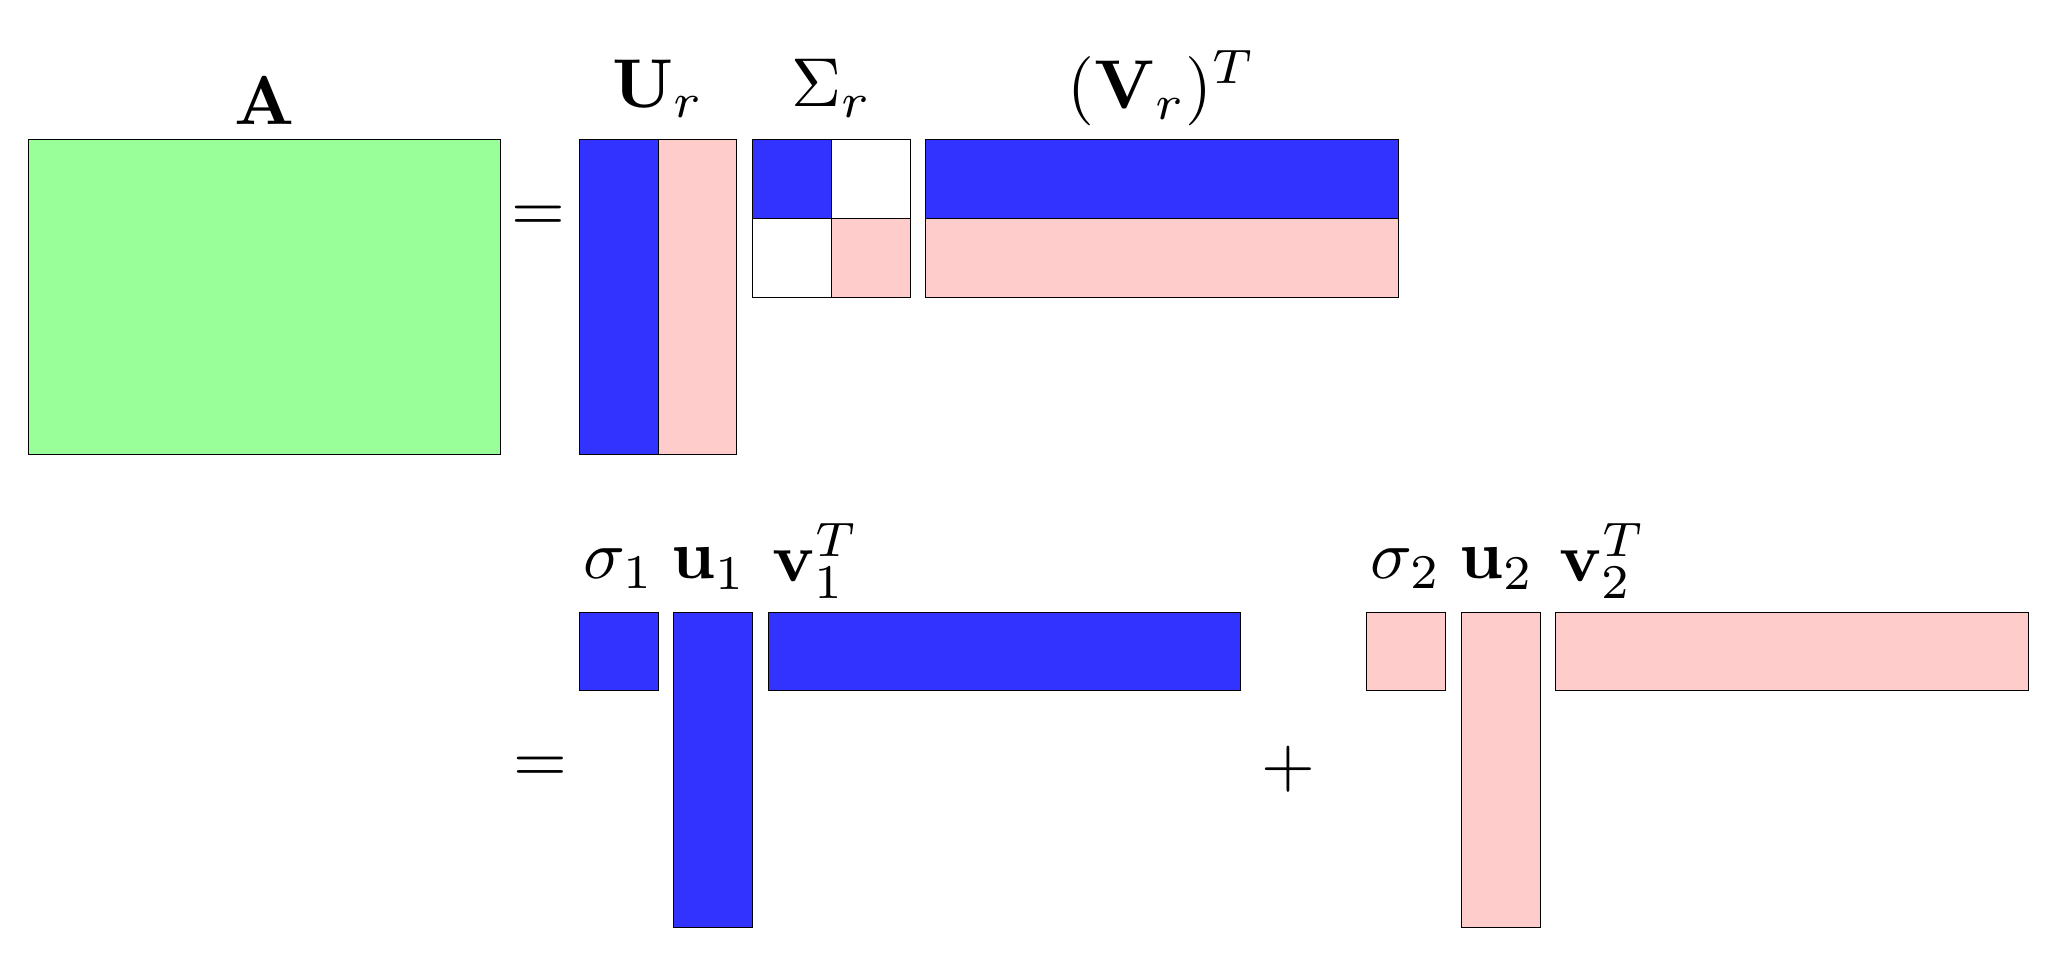
\begin{tikzpicture}
    \def\m{4}
    \def\n{6}
    \def\r{2}
    \begin{scope}
        \node [scale = 2.5] at (0.5*\n, 0.5) {$\mathbf{A}$};
        \draw [fill = green!40] (0, 0) rectangle (\n, -\m);
        \node [scale = 2.5] at (1.08*\n, -0.25*\m) {$=$};
    \end{scope}

    \begin{scope}[xshift = 7cm]
        \node [scale = 2.5] at (1, 0.65) {$\mathbf{U}_r$};
        
        \draw [fill = blue!80] (0, 0) rectangle (1, -\m);
        \draw [fill = red!20] (1, 0) rectangle (2, -\m);
    \end{scope}

    \begin{scope}[xshift = 9.2cm]
        \node [scale = 2.5] at (1, 0.65) {$\Sigma_r$};
        \draw [fill = blue!80] (0, 0) rectangle (1, -1);
        \draw [fill = red!20] (1, -1) rectangle (2, -2);
        \draw (0, 0) rectangle (2, -2); 
    \end{scope}

    \begin{scope}[xshift = 11.4cm]
        \node [scale = 2.5] at (.5*\n, 0.65) {$(\mathbf{V}_r)^T$};
        \draw [fill = blue!80] (0, 0) rectangle (\n, -1);
        \draw [fill = red!20] (0, -1) rectangle (\n, -2);
    \end{scope}

    \begin{scope}[xshift = 7cm, yshift = -6cm]
        \node [scale = 2.5] at (.5, .55) {$\sigma_1$};
        \node [scale = 2.5] at (1.65, .55) {$\mathbf{u}_1$};
        \node [scale = 2.5] at (3, .65) {$\mathbf{v}^T_1$};

        \draw [fill = blue!80] (0, 0) rectangle (1, -1);
        \draw [fill = blue!80] (1.2, 0) rectangle (2.2, -\m);
        \draw [fill = blue!80] (2.4, 0) rectangle (\n + 2.4, -1);
        \node [scale = 2.5] at (1.5*\n, -0.5*\m) {$+$};
        \node [scale = 2.5] at (-.5, -0.5*\m) {$=$};
        \begin{scope}[xshift = 10cm]
            \node [scale = 2.5] at (.5, .55) {$\sigma_2$};
            \node [scale = 2.5] at (1.65, .55) {$\mathbf{u}_2$};
            \node [scale = 2.5] at (3, .65) {$\mathbf{v}^T_2$};

            \draw [fill = red!20] (0, 0) rectangle (1, -1);
            \draw [fill = red!20] (1.2, 0) rectangle (2.2, -\m);
            \draw [fill = red!20] (2.4, 0) rectangle (\n + 2.4, -1);
        \end{scope}        
        
    \end{scope}


\end{tikzpicture}
\end{document}